\renewcommand*{\arraystretch}{1.1}

\subsection*{BI / read / 10}
\label{section:bi-read-10}

% change \emph{} to use sans-serif font
\let\oldemph\emph
\renewcommand{\emph}[1]{{\footnotesize \sf #1}}

\renewcommand{\currentQueryCard}{10}
\marginpar{
	\raggedleft
	\vspace{0.22ex}

	\queryRefCard{bi-read-01}{BI}{1}\\
	\queryRefCard{bi-read-02}{BI}{2}\\
	\queryRefCard{bi-read-03}{BI}{3}\\
	\queryRefCard{bi-read-04}{BI}{4}\\
	\queryRefCard{bi-read-05}{BI}{5}\\
	\queryRefCard{bi-read-06}{BI}{6}\\
	\queryRefCard{bi-read-07}{BI}{7}\\
	\queryRefCard{bi-read-08}{BI}{8}\\
	\queryRefCard{bi-read-09}{BI}{9}\\
	\queryRefCard{bi-read-10}{BI}{10}\\
	\queryRefCard{bi-read-11}{BI}{11}\\
	\queryRefCard{bi-read-12}{BI}{12}\\
	\queryRefCard{bi-read-13}{BI}{13}\\
	\queryRefCard{bi-read-14}{BI}{14}\\
	\queryRefCard{bi-read-15}{BI}{15}\\
	\queryRefCard{bi-read-16}{BI}{16}\\
	\queryRefCard{bi-read-17}{BI}{17}\\
	\queryRefCard{bi-read-18}{BI}{18}\\
	\queryRefCard{bi-read-19}{BI}{19}\\
	\queryRefCard{bi-read-20}{BI}{20}\\
	\queryRefCard{bi-read-21}{BI}{21}\\
	\queryRefCard{bi-read-22}{BI}{22}\\
	\queryRefCard{bi-read-23}{BI}{23}\\
	\queryRefCard{bi-read-24}{BI}{24}\\
	\queryRefCard{bi-read-25}{BI}{25}\\
}


\noindent\begin{tabularx}{\queryCardWidth}{|>{\queryPropertyCell}p{\queryPropertyCellWidth}|X|}
	\hline
	query & BI / read / 10 \\ \hline
%
	title & Central Person for a Tag \\ \hline
%
	pattern & \hfill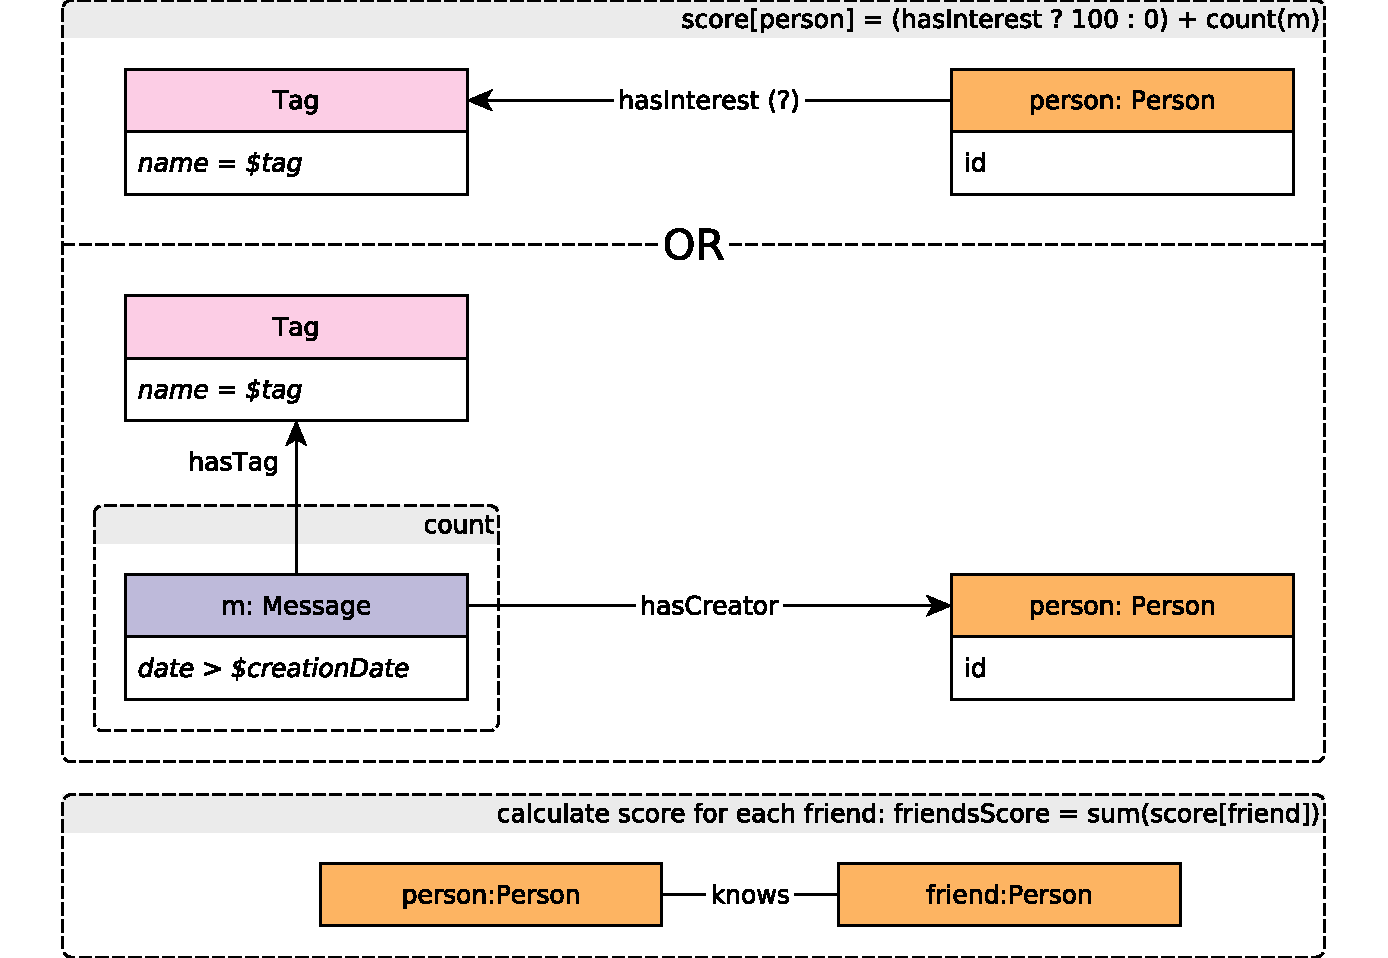
\includegraphics[scale=\patternscale,margin=0cm .2cm]{patterns/bi-read-10}\hfill\vadjust{} \\ \hline
%
	desc. & Given a \emph{Tag}, find all \emph{Persons} that are interested in the
\emph{Tag} and/or have written a \emph{Message} (\emph{Post} or
\emph{Comment}) with a \texttt{creationDate} after a given \texttt{date}
and that has a given \emph{Tag}. For each \emph{Person}, compute the
\texttt{score} as the sum of the following two aspects:

\begin{itemize}
\tightlist
\item
  100, if the \emph{Person} has this \emph{Tag} as their interest, or 0
  otherwise
\item
  number of \emph{Messages} by this \emph{Person} with the given
  \emph{Tag}
\end{itemize}

Also, for each \emph{Person}, compute the sum of the score of the
\emph{Person}'s friends (\texttt{friendsScore}).
 \\ \hline
%
	
		params &
		\innerCardVSpace{\begin{tabularx}{\attributeCardWidth}{|>{\paramNumberCell}c|>{\varNameCell}M|>{\typeCell}m{\typeWidth}|Y|} \hline
		$\mathsf{1}$ & tag
 & String
 &  \\ \hline
		$\mathsf{2}$ & date
 & Date
 &  \\ \hline
		\end{tabularx}}\innerCardVSpace \\ \hline
	
%
	
		result &
		\innerCardVSpace{\begin{tabularx}{\attributeCardWidth}{|>{\resultNumberCell}c|>{\varNameCell}M|>{\typeCell}m{\typeWidth}|>{\resultOriginCell}c|Y|} \hline
		$\mathsf{1}$ & person.id & 64-bit Integer & R &
				 \\ \hline
		$\mathsf{2}$ & score & 32-bit Integer & A &
				 \\ \hline
		$\mathsf{3}$ & friendsScore & 32-bit Integer & A &
				The sum of the score of the Person's friends
 \\ \hline
		\end{tabularx}}\innerCardVSpace \\ \hline
	
%
	
		sort		&
		\innerCardVSpace{\begin{tabularx}{\attributeCardWidth}{|>{\sortNumberCell}c|>{\varNameCell}M|>{\directionCell}c|Y|} \hline
		$\mathsf{1}$ & score + friendsScore
 & $\desc
$ &  \\ \hline
		$\mathsf{2}$ & person.id
 & $\asc
$ &  \\ \hline
		\end{tabularx}}\innerCardVSpace \\ \hline
	%
	limit & 100 \\ \hline
	%
	CPs &
	\multicolumn{1}{>{\raggedright}l|}{
		\chokePoint{1.2}, 
		\chokePoint{2.1}, 
		\chokePoint{2.3}, 
		\chokePoint{3.2}
		} \\ \hline
	%
	%
\end{tabularx}
\queryCardVSpace

% change \emph back to the old one
\renewcommand{\emph}[1]{\oldemph{#1}}